\part{Routine Development}
	From very early on I recognized that a RoboCup Dance \index{routine}routine had to have an interesting routine. It's not all about tech, it's also about the \index{entertainment}entertainment factor.\\
    
    For each level of the competition I have developed a different routine. I always had in mind that I wanted some sort of \index{story}\index{storyline}\hyperref[Story]{storyline} to the performance to provide interest, and draw the audience in. For \index{regionals}Regionals and \index{states}States I didn't create a particular \hyperref[Story]{storyline}, but for \index{nationals}Nationals I've been able to implement a good \hyperref[Story]{storyline}.\\
    
    For Regionals I had a \index{Christmas}Christmas \index{theme}theme, using a \index{Christmas Tree}Christmas tree and presents as props. I animated the \index{regionals}Regionals Routine in around 2 days. I was animating the lights and Christmas tree up until the night before. I feel that the Regionals performance has been the best to date.\\
    
    For \index{States}States I had no particular theme. I didn't really like the States \index{routine}routine - it felt too much like a mashpot of random things that were disjointed and didn't fit together. I feel the reason for this is that I had created the \index{stage}"Stage" \hyperref[Props]{prop} and based the routine around the stage \index{stage}"Stage" \hyperref[Props]{prop}, rather than basing the prop around the routine. It felt rather disjointed, and didn't flow. Rather than the \index{stage}"Stage" \hyperref[Props]{prop} adding to the performance, I felt it subtracted from it. Along with this I had only allowed myself a day to animate the robot, which was not enough to produce a quality performance. You may be wondering why 1-2 days was enough for \index{regionals}Regionals, but not for States - and it's because for Regionals I had the benefit of months to think about what I was going to animate, before \index{animating}animating it. For states I had to come up with what I wanted to animate, and animate it within a day.\\
    
    For Nationals I have a very specific \index{storyline}\hyperref[Story]{storyline}. In essence the \index{nationals}Nationals routine is the essence of what I wanted my routine to always be like. The performance tells a story of a robot and it's creator - a story of \index{rejection}rejection and \index{reconciliation}reconciliation. After the \index{states}states. \\
    
    	\section{Parts of a Routine}
    	There are many parts that go into a RoboCup Junior \index{Dance}Dance \index{routine}routine, each are incredibly significant - and whilst by themselves they may not seem particularly significant, as a whole they make up a polished routine.\\
        
        These parts include Audio, Robot Performance/Animation, Human Performance, Props, Story, Stage and Presence/Audience Interactivity.\\
        
        It's important to keep all these factors in mind whilst developing a routine - to gain the most optimal result.\\
        
        
        
        
    
    	\chapter{Audio}
    	\section{Audio Uses}
        \index{audio}
        \index{audio uses}
          Audio is obviously one of the more important parts of the routine. It can convey significant emotion that the robot by itself cannot. Many times I show people my robot doing a RoboCup performance - but the performance is rather dry in of itself, because the Audio really enhances and provides an explanation to what the robot is doing.\\
        
          The real advantage with the way I constructed the robot's development environment is that I can very accurately animate the robot to the music. This \index{synchronization}\index{sync}synchronization between the robot and the \index{music}music can be used with great effect together.\\
          
          I've also been able to leverage the sync advantage by adding in \index{sound effects}sound effects to the track - such as a roar, and then having the robot roar in sync to the effect. I've also been able to use other effects, such as having the robot sigh, and use "robot motor sounds" to exaggerate it's movement effect.\\
          
          Obviously audio can also be used to tell a \hyperref[Story]{story}, as I'm doing in Nationals. I was inspired by using short snippets of music to tell a \hyperref[Story]{story} by the following \textit{Britain's Got Talent} act:\\
          
          \url{https://www.youtube.com/watch?v=FP7wN301yjc}\\
          
			I didn't want to be restricted to one song - or even one genre in my performances, and that's why I opt to use a mix of songs. Especially at \index{regionals}Regional level people commented that using different genre of music in the performance, in a short period of time really showed off the strengths of the robot - in it's timelessness. Another advantage of using different genres of music is that if one particular song doesn't appeal to some members of the audience, the next genre might.\\
            
            
		\section{Audio Selection}
        	\label{sec:audio_selection}
            \index{audio selection}
        	For every 10 people choosing music for a RoboCup \index{routine}Routine, you'll get 11 different opinions. Because of this I have determined that whilst it's wise to listen to all opinions, ultimately I need to make the decision based upon what I like. Often if I like the selection of \index{audio}audio, in the end, other people do too.\\
            
            On occasions I have selected music or sound effects that didn't particularly compliment the performance, and more than often other people warned me of this. Typically these are small things though, and overall the selection of audio has been complimented. For final decision making, I take other peoples views, consider them, and then make the final decision based upon what I like.\\
            
            I have found that well known music with a beat are typically the favorites. Examples of these are \textit{Gangnam Style - Psy}, \textit{I Feel Good - James Brown}, and \textit{Stayin' Alive - Beegees}. On the other hand, audio such as \textit{Pink Panther Theme}, and \textit{Baby - Justin Bieber} weren't nearly as popular. If it's something you can tap your feet to, it's something that'll work.\\
            
            This is what has caused me the most worry about my \index{nationals}Nationals \index{music}music selection. I've picked a mixture of music that has a good beat, popular, and wel known - but my entire routine is not comprised of it. For example, my opening song for Nationals, \textit{Create/Destroy - Art vs. Science}, is not well known, however has a good beat (and I really like it). \textit{All By Myself - Celion Dion} is well known, but doesn't have as much of a beat. I'm mainly worried because I have none of the songs that have proven their worth previously (Gangnam Style, I Feel Good, Stayin' Alive, etc).\\
            
            This being said, the purpose of this routine isn't to get the audience bobbing their heads - but rather to convey a story, which I feel the selection of music does amply. In short, I'm taking a risk by experimenting - but I think it'll pay off. In the past at Regionals and States my experimentation has typically paid off in my routine being quite unique.\\
            
            \index{final audio selection}
            That being said, here's the final selection of music for Nationals (in order):\\
            
            \begin{enumerate}
            	\item Create/Destroy - Art vs. Science
                \item Clocks - Coldplay
                \item Beat it - Michael Jackson
                \item All by Myself - Celion Dion
                \item Circle of Life - Lion King Theme
            \end{enumerate}
            
		\section{Audio Editing}
        	\index{audio editing}
            \label{audio_editing}
        	If I'm to have multiple songs in the routine, then I need some way to cut them all together. For Regionals and States I used \index{Audacity}Audacity. For Nationals I moved to using \index{Adobe}\index{Adobe Audition}Adobe Audition. Both these are fantastic tools, and a pleasure to learn. Although I'm not particularly skilled in Audio editing, I have did a short course on a camp once, the knowledge of which I was able to employ.\\
            
            \centerline{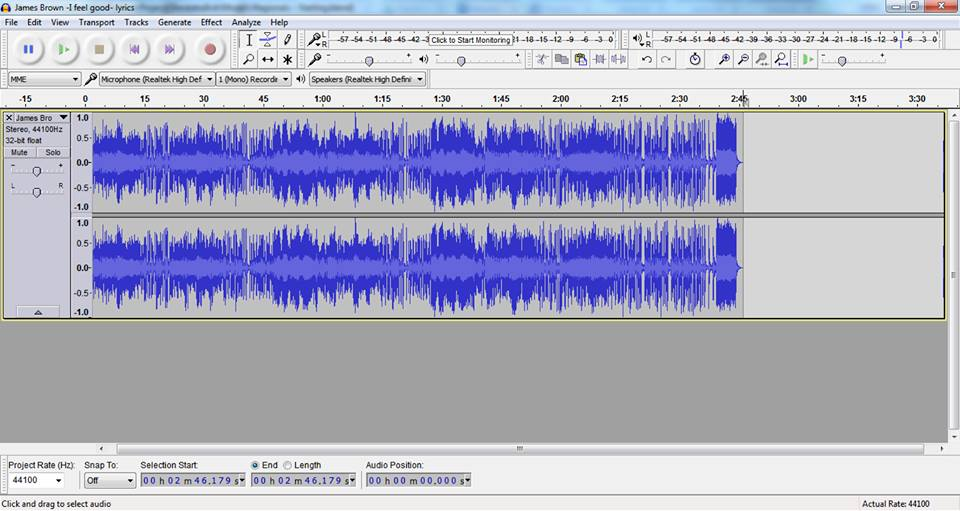
\includegraphics[width=0.75\linewidth]{images/audio_editing}}
            \vspace{10pt}
            
            \centerline{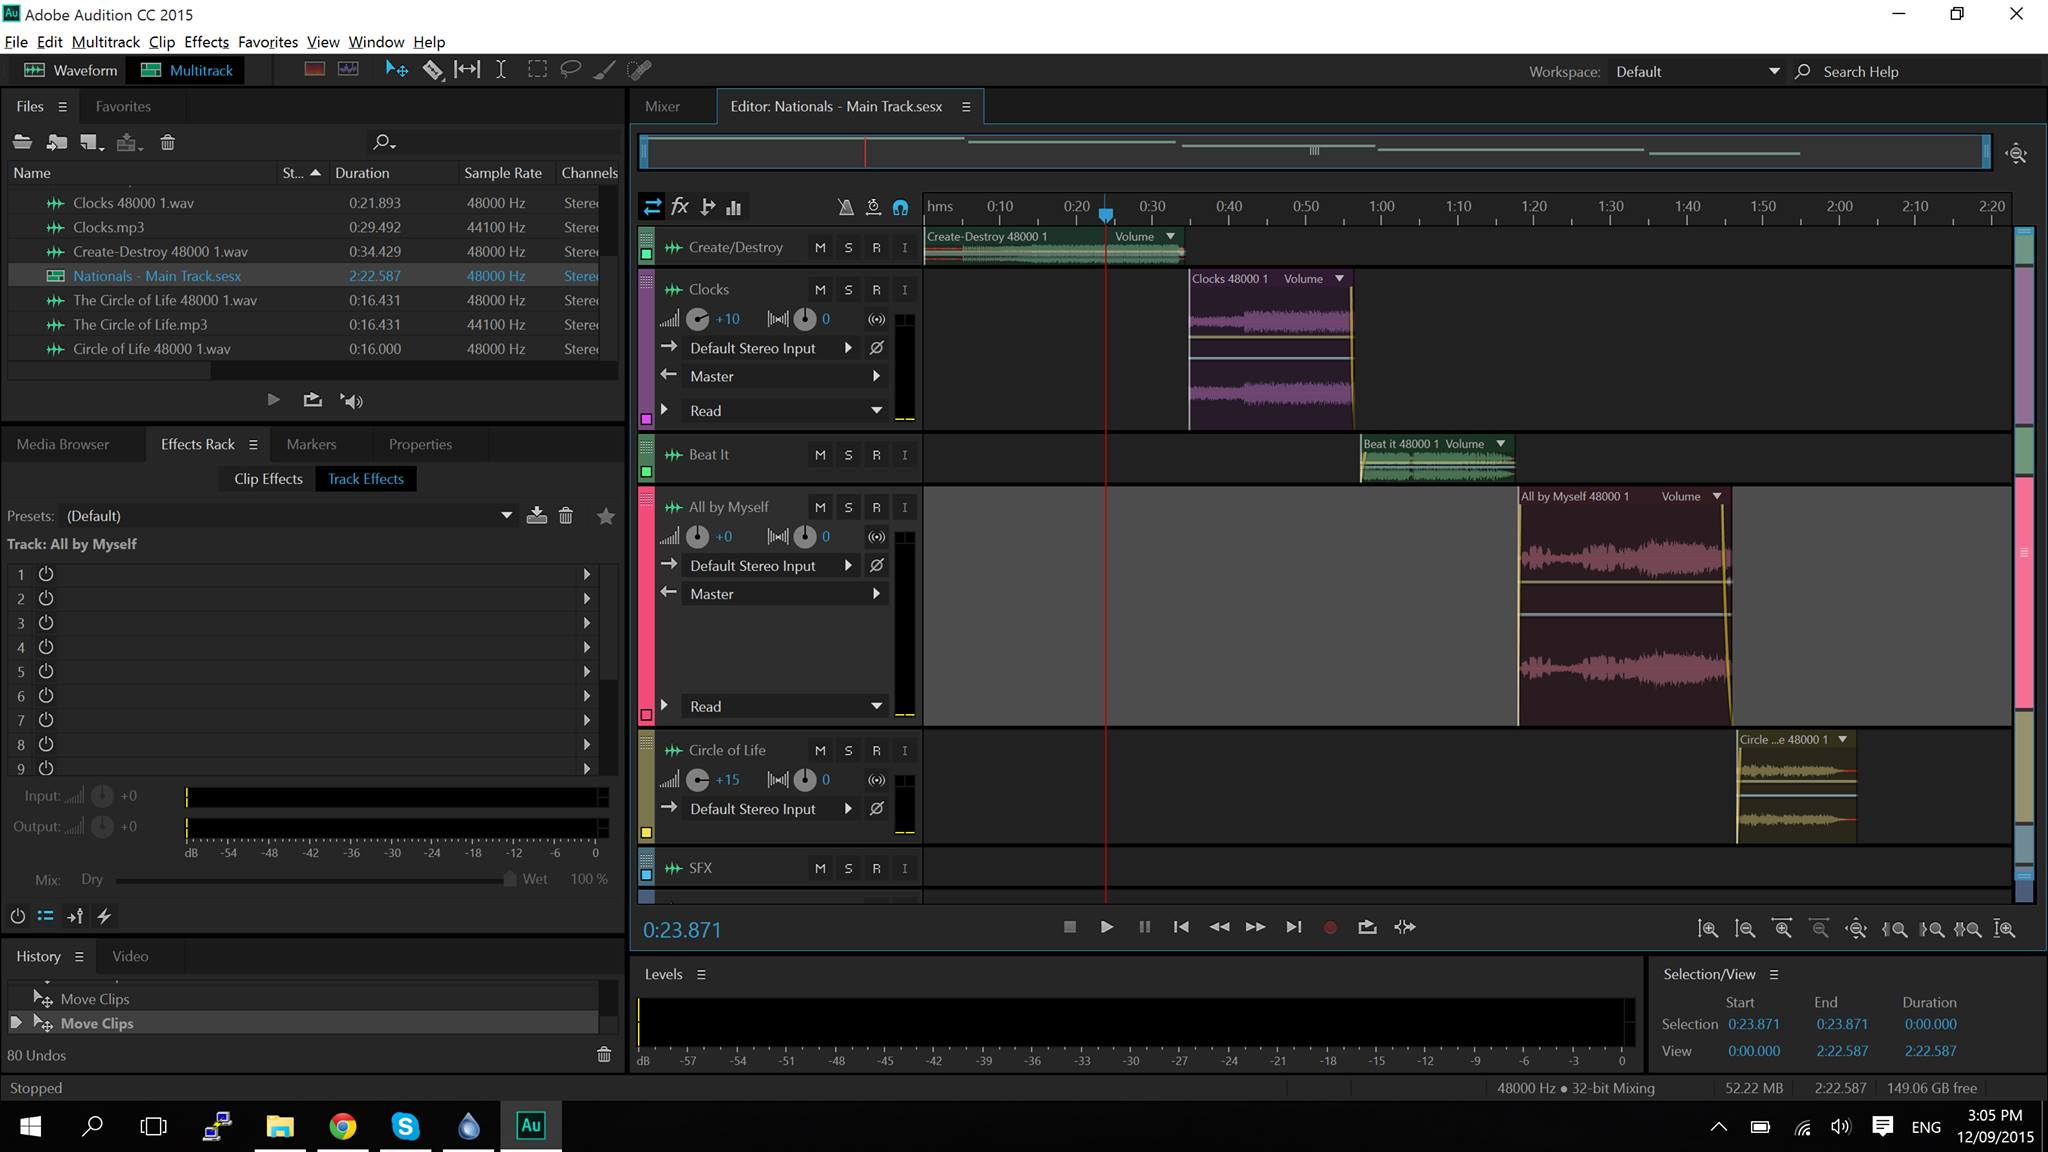
\includegraphics[width=0.75\linewidth]{images/audition_audio_editing}}
            \vspace{10pt}                        
            
            The biggest problem in editing songs together is figuring out when and how to cut a song. Obviously I can't string 5 full length songs together, so I need to cut out the parts I want. Typically I like to keep each individual song to 20-30 seconds each. I try to find a place which I can cut it in that vicinity.\\
            
            I employ two major techniques to gain a cleaner cut if where I'm cutting the song is not clean in of itself:\\
            
            \subsection{Fade In/Fade Out}
            	This one is somewhat self explanatory, fading in and out is a great way to soften unclean cuts.\\
                
			\subsection{Cutting Parts of the Song Together}
            	Sometimes you're able to cut the beginning of a song to the end. The advantage of this is that you get a clean start (as you are using the start of the song), and a clean end (because you are using the actual end of the song). If you are very careful, you are able to get these two cuts and combine them with no noticeable cut.\\
                
                An example of when I used this was in the \textit{I Feel Good} audio. I cut the start of the song, straight to the end - cutting out the middle lyrics and chorus. I cannot distinguish where I have cut the music together - even when I'm looking for it, so the audience doesn't suspect a thing.\\      
                
		                
                
            
            
            

    
    	\chapter{Robot Performance/Animation}
		The way that I designed the development environment for the hexapod, I am able to animate the routine to the music using the open-source 3D modeling and animation software, Blender.\\
        
        \section{Animation}
        
          To give you the best overall idea of what the process of animating the robot looks like, I've compiled a stopmotion video of me animating a movement. This particular movement was for States, and I was animating the robot stepping off a raised platform, onto the ground. This took around 2 hours for me to animate.\\

          \url{https://www.youtube.com/watch?v=o0-15CS6urg}\\

          All things considered animation isn't the most time consuming activity, but I might venture to say that it is the most irritating. Often you are listening to the same music over and over, and doing very repetitive tasks. Often you have to delete half an hours worth of work at a time. It's not uncommon to throw away several seconds of content (which could have taken hours to create).\\

          You can do many things when animating that won't work in real life - you can make the robot jump in Blender, but that doesn't mean the robot will jump in real life. You need to have a good sense of how the robot works, physically, to be able to animate it. This is not all bad though - if you are familiar with what the robot will do in regards to how you animate it in Blender, you can achieve some pretty amazing results that you wouldn't normally be able to achieve if you animated the robot conventionally.\\

          The soundtrack has to be fully created before starting animation, as I animate to the music. To do this I add the soundtrack to the timeline in Blender, allowing me to hear the audio whilst I'm animating, allowing me to animate to the music.\\

          \centerline{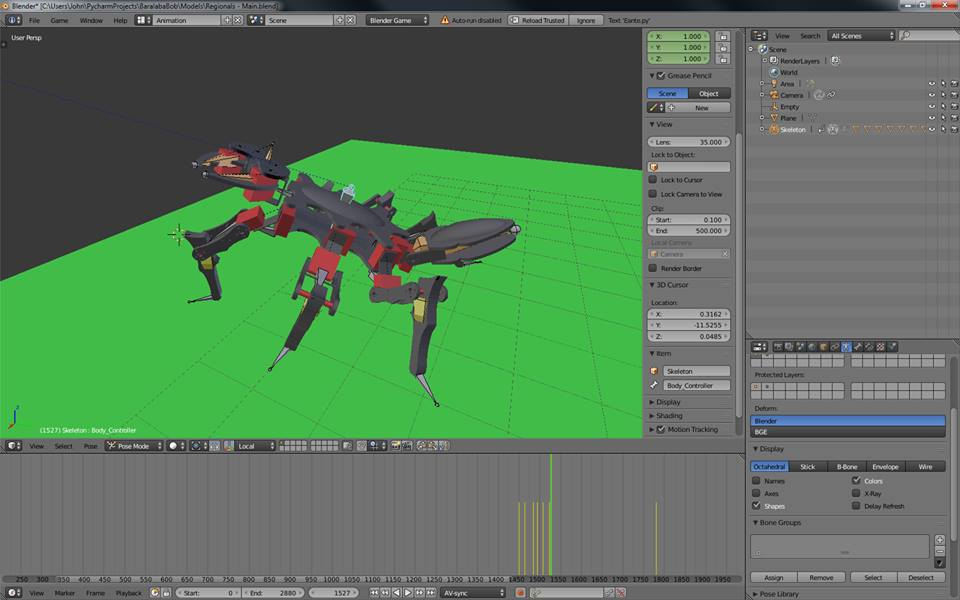
\includegraphics[width=\linewidth]{images/animation}}
          \vspace{10pt}
          \centerline{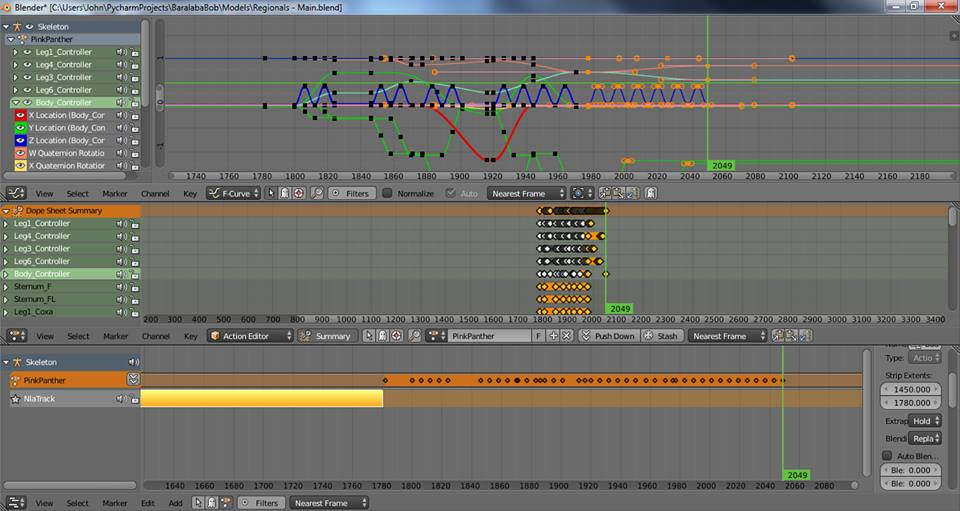
\includegraphics[width=\linewidth]{images/graph_editor}}
          \vspace{10pt}
          
          
         \index{unique}
		\section{Performance}
        	Before animating the routine for \index{regionals}Regionals, I had thought of a lot of movements which I could put to music - allowing me to develop them quickly. For \index{states}States I hadn't thought of movements - I was animating and making up movements on the fly.\\
            
			Some considerations in the development of the \index{robot}robot's routine is making sure I use as much of the \index{floor space}floor space as possible, having lots of \index{unique movements}unique movements to maintain interest, making sure the movements fit the audio, and ensuring that the movements aren't straining the robot \index{motor failure} (causing motor failure).\\
            
            \textit{\textbf{Also see: }\hyperref[motor_failure]{Motor Failure}}
            
            It's very difficult to walk the robot around the entire floor space, as it takes a while to have the robot walk anywhere. Part of this is my not wanting to strain the robot by having it walk fast, but as time goes on I get more and more adventurous with how far I push the robot. The problem of \index{movement speed}movement speed still presents itself.\\
            
            One of the sub-difficulties is that turning the robot is very slow. It takes a minimum of 3-4 individual turn sequences on the robot to turn a full 90 degrees, each turn taking 0.5-2 seconds. Multiply 4 by 2 seconds, and you quickly run into a very time consuming movement, at 8 seconds - and that's just to turn 90 degrees. I prefer to have the robot walk sideways, than turning sideways and then walking in that direction. The advantage of a legged base is that you don't have to face the direction you walk, so you can do this.\\
            
            Having unique movements to provide interest isn't particularly difficult to create, but it is often difficult to animate and time consuming to integrate into the routines. It often takes many hours of continuous effort to animate a single 10-15 second segment.\\
            
            

        
        
    	
    
    	\chapter{Human Performance}
    	From the outset I realized that a good performance will include good \index{human interaction}human interaction. As expressed in the Dance Performance score sheet, the interaction should not detract from the robot itself - but I believe a performance can be rounded off with a good human performance.\\
        
        I'm naturally not a person who defaults to dancing or acting on stage - however because of requirement to do so, I recognized that I needed to put aside my illogical fears, and perform. The result of this is that I made an agreement with myself that I would put aside any fears or doubts about performing on stage, and that I was just do what I had to do, and put my all into it.\\
        
        I believe that because I made this agreement with myself, I was able to give a half decent performance, which compliments the robot. As I've mentioned previously, I don't want to detract from robot's performance, but at the same time I try to create a human-robot interaction throughout the performance in the setting of a story to increase the entertainment factor.\\
        
        Often my performance comes from what I want the robot to do. Often the comical factor of the robot is it showing attitude to me. It's quite simple to express emotion in reaction to the robot. For example, I can look surprised when the robot roars at me. Just having the robot perform is only one side of a conversation - having a robot respond to the robot adds the second side of the conversation.\\
        
        \section{Human Interaction Incidence}
        	\index{human_interaction}
        	There was one incident at State titles which caused a problem I hadn't anticipated. The issue was that how my routine was developed, I would stand to the left of the robot for the duration of the routine - as the robot would face me at times throughout the routine (ex. roaring at me).\\
            
        	On the day, I didn't have a good way of solving this problem (except for standing on the other side of the performance, and hope for the best), which is what I did.\\
            \index{judges}
            For \index{nationals}Nationals I'm conscious of this problem, but as of yet haven't found a suitable solution. The best solution is to create two instances of the performance - one for right side, and one for left. Unfortunately this effectively doubles my work, which I may not have time to do. I have a theory that I \textit{may} be able to "mirror" the actions in blender, and export the mirror, but I haven't been able to test this yet.\\
            
            For Nationals I will advise the judges previously to the nature of the positioning of the \index{routine}routine, and also I'll try to keep out of their view as much as possible.\\
            
			\section{Stage Presence/Audience Interactivity}
    	Having good stage presence can also really round out a routine. Having stage presence means that you are able to command and hold the attention of the audience, simply by your demeanor and confidence. This can be achieved by confidently introducing your routine, and talking directly to the audience.\\
        
        Audience Interactivity can include asking the audience to clap along, sing, or maybe even dance! This helps draw the \index{audience}audience in, and creates a fun and vibrant atmosphere. I employed asking the audience to clap along for \index{regionals}Regionals and States. Because I'm doing a different kind of routine for Nationals, I'm not sure if I am able to include this kind of interactivity.\\
        
        
            
            
        
        
    
    	\chapter{Props}
    	\label{Props}
        \index{props}
    	Props are to enhance a routine. This is a fatal mistake I made in States.\\
        
        For \index{regionals}Regionals in \index{Rockhampton}Rockhampton, I designed the entire \index{Christmas}Christmas routine, including \index{audio}audio, \index{animating}animating, etc. All the while I was thinking about what props I could use to enhance the routine. This worked really well, and I got a lot of really good props I used to great effect.\\
        
        However, for States I got caught up in trying to create excellent props. The result was that I got a really good \index{stage}"stage" prop - but I put all my time into designing the props, and not enough into routine development. The result was that I created the routine around the props, and not around the music or story.\\
        
        This meant I couldn't \index{animate}animate the routine as well as I wanted, and the story/routine was disjointed and not flowing. I learned my lesson from this, and for \index{nationals}Nationals I have put my efforts into creating the routine.\\
        
        I've found that as I create the routine, I naturally think of funny and engaging props that will enhance the show. When it comes time to adding props, I don't have to put too much effort in, as I already know what I want.\\
        
        For Nationals I had created the \index{story}\hyperref[Story]{storyline} that I wanted and as I was working on animating I realized that having a lab-coat, safety glasses, misc tools scattered around, and some technical panel with dials, buttons, and lights would enhance the routine. Most of these things I have lying around at home, and I can easily put them on a plane.\\
        
        The only thing I'm thinking of working on is the panel with lights and stuff. I put a few hours aside for creating something like that, and programming it.\\
        
        
    
    	\chapter{Story}
    	\label{Story}
		I'm a big believer in adding a story to most anything. I think stories engage the \index{audience}audience, and draw them in. It creates an emotional attachment to the performance, and to the actors. I like to employ stories and storytelling in things I teach, and performances I put on.\\
        
        The story of this performance is loosely modeled after the story of the Prodigal Son in Luke 15:11-12 (The Bible) - and typically the creation/salvation story outlined in the Bible.\\
        
        In the story, I'm the creator/father figure, and I create my son/child/robot. We are at first having fun, and enjoying each other's company - but as time goes by the robot gets annoyed, and pushes me away. The robot walks off, but through which time the father wishes that his son was with him all the while. The father doesn't care that his son did him wrong - his love transcends that sin.\\
        
        After a while, the robot realizes that he was better off, and happier with his creator. They both come back together again, and lived happily ever after!\\              
    
    
    
    
    
    